\subsection{Color Mixing}

I diagrammet, Figur~\ref{fig:chromaticity-diagram} kan en ret linje mellem to punkter (farver) viser alle de mulige farver som kan genereres ved at blade de to farver (punkter),

\begin{figure}[H]
	\centering
	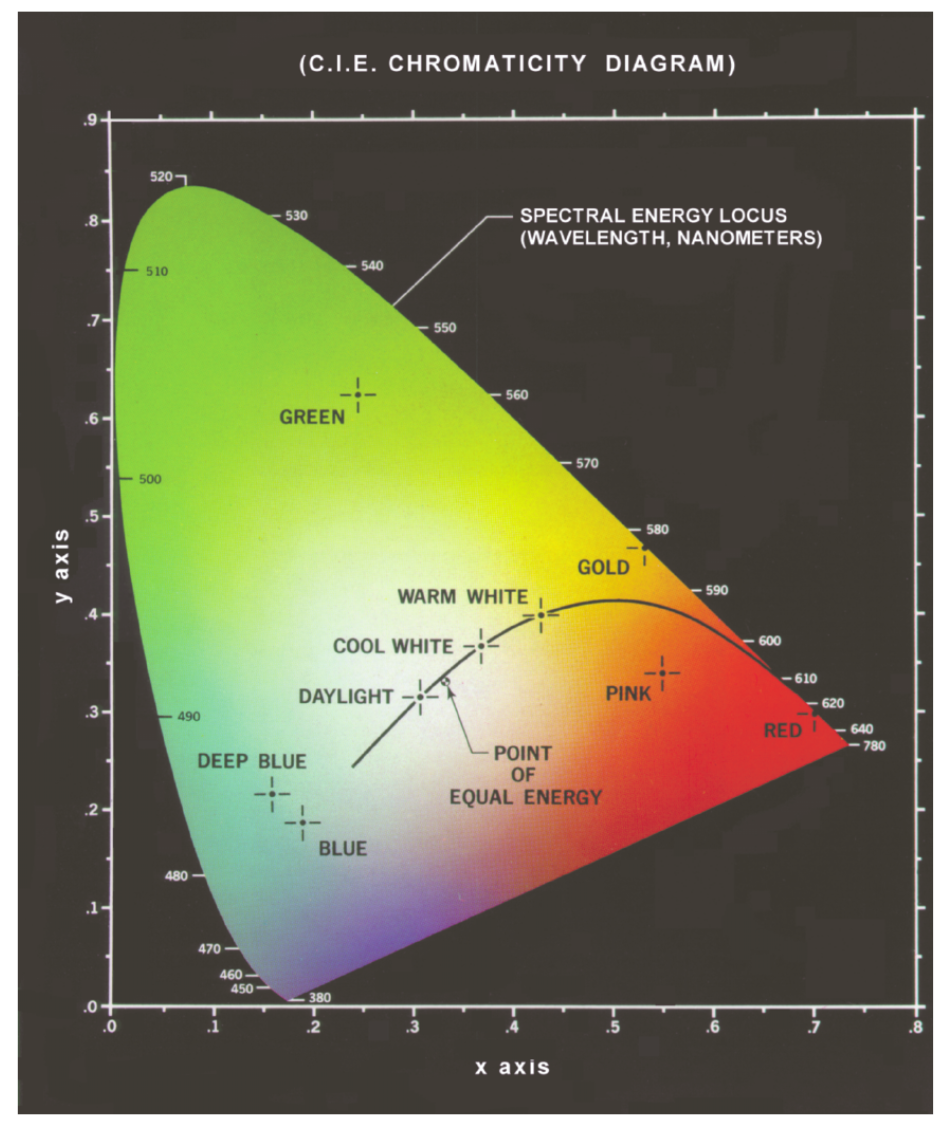
\includegraphics[width=0.7\linewidth]{figs/spm07/chromaticity-diagram}
	\caption{Chromaticity diagram.}
	\label{fig:chromaticity-diagram}
\end{figure}

Figur~\ref{fig:rgb-color-cube} viser farveterningen hvor de primær og sekundære farver.

\begin{figure}[H]
	\centering
	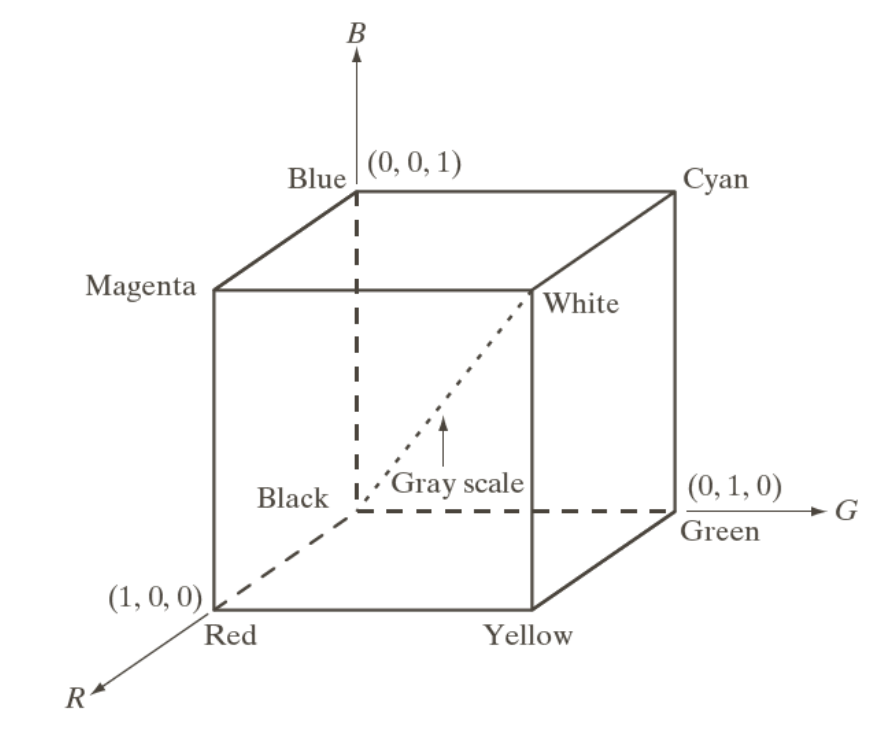
\includegraphics[width=0.7\linewidth]{figs/spm07/rgb-color-cube}
	\caption{RGB color cube.}
	\label{fig:rgb-color-cube}
\end{figure}
